\documentclass[9pt]{article}
\usepackage[landscape,a4paper,top=0.5cm,bottom=0.5cm,left=0.6cm,right=0.6cm]{geometry}
\usepackage{graphicx}
\usepackage{amsmath,amssymb}
\usepackage{booktabs}
\usepackage[most]{tcolorbox}
\usepackage{xcolor}
\usepackage{microtype}
\usepackage{tabularx}
\usepackage{hyperref}
\usepackage{enumitem}

\pagestyle{empty}

% Color Palette
\definecolor{spaceNavy}{HTML}{0B192C}
\definecolor{headerNavy}{HTML}{1E293B}
\definecolor{electricCyan}{HTML}{0284C7}
\definecolor{lightCyan}{HTML}{E0F2FE}
\definecolor{darkCyan}{HTML}{0369A1}
\definecolor{accentAmber}{HTML}{D97706}
\definecolor{lightAmber}{HTML}{FEF3C7}
\definecolor{cardBg}{HTML}{FFFFFF}
\definecolor{cardBorder}{HTML}{CBD5E1}
\definecolor{textDark}{HTML}{0F172A}
\definecolor{textMuted}{HTML}{475569}
\definecolor{pillBg}{HTML}{1E293B}
\definecolor{pillCyan}{HTML}{0EA5E9}
\definecolor{greenAccent}{HTML}{16A34A}
\definecolor{redAccent}{HTML}{DC2626}

% Custom tcolorbox styling
\tcbset{
    posterbox/.style={
        enhanced,
        colback=white,
        colframe=cardBorder,
        boxrule=1pt,
        arc=4pt,
        left=6pt,right=6pt,top=5pt,bottom=5pt,
        fonttitle=\bfseries\small,
        coltitle=white,
        colbacktitle=spaceNavy,
        titlerule=0pt,
        boxsep=2pt
    },
    highlightbox/.style={
        enhanced,
        colback=lightCyan!40,
        colframe=electricCyan,
        boxrule=1pt,
        arc=3pt,
        left=5pt,right=5pt,top=4pt,bottom=4pt,
        boxsep=2pt
    },
    amberbox/.style={
        enhanced,
        colback=lightAmber!40,
        colframe=accentAmber,
        boxrule=1pt,
        arc=3pt,
        left=5pt,right=5pt,top=4pt,bottom=4pt,
        boxsep=2pt
    }
}

\begin{document}

% ==============================================================================
% PAGE 1: THE PROBLEM, THE DES DILEMMA, AND ARCHITECTURAL SOLUTION
% ==============================================================================

% Header Banner Page 1
\begin{tcolorbox}[enhanced, colback=spaceNavy, colframe=electricCyan, boxrule=1.5pt, arc=5pt,
    left=9pt, right=9pt, top=5pt, bottom=5pt]
    \begin{minipage}[c]{0.74\textwidth}
        {\fontsize{7.5pt}{9pt}\selectfont \color{electricCyan}\textbf{INTERNATIONAL CONFERENCE ON NS-3 (ICNS3 - 2026) --- LIGHTNING TALK}}\\[2pt]
        {\fontsize{13pt}{15pt}\selectfont \color{white}\textbf{The Limits of Discrete-Event Schedulers in Interplanetary Network Simulation:}}\\[1pt]
        {\fontsize{11pt}{13pt}\selectfont \color{pillCyan}\textbf{Why Deep Space Breaks Conventional DES Paradigms}}\\[3pt]
        {\fontsize{8pt}{10pt}\selectfont \color{gray!30}\textbf{Jason Pandian} (\textit{Presenter}, \texttt{pandiajason@gmail.com})\\
        \textit{Department of Information Technology, Nehru Institute of Technology, Coimbatore, India}}
    \end{minipage}%
    \hfill
    \begin{minipage}[c]{0.24\textwidth}
        \centering
        \begin{tcolorbox}[colback=pillBg, colframe=electricCyan, boxrule=0.8pt, arc=3pt, left=4pt, right=4pt, top=3pt, bottom=3pt]
            \centering
            {\fontsize{7pt}{8pt}\selectfont \color{pillCyan}\textbf{FOCUS: DES ARCHITECTURE CRITIQUE}}\\[1pt]
            {\fontsize{6.5pt}{7.5pt}\selectfont \color{white} Multi-Minute Delay vs. Frozen Events}\\
            {\fontsize{6.5pt}{7.5pt}\selectfont \color{white} Continuous Orbits vs. Event Queues}\\
            {\fontsize{6.5pt}{7.5pt}\selectfont \color{lightAmber}\textbf{Mode: Virtual Presentation}}
        \end{tcolorbox}
    \end{minipage}
\end{tcolorbox}

\vspace{0.1cm}

% 3-Column Layout Page 1
\begin{minipage}[t]{0.32\textwidth}
    \begin{tcolorbox}[posterbox, title=1. The Deep-Space Simulation Challenge, height=15.2cm]
        {\color{darkCyan}\textbf{How Terrestrial Simulators Work (e.g., ns-3):}}
        \begin{itemize}[leftmargin=9pt, itemsep=1.5pt, topsep=1pt]
            \item \textbf{Event-Driven Clock:} Traditional network simulators sleep until a packet is sent or received (a discrete ``event'').
            \item \textbf{Instant Signals:} On Earth, radio waves travel almost instantly (a few milliseconds across continents). Nodes are assumed to stay put or move predictably during packet exchange.
            \item \textbf{Great for Earth:} Highly effective for Wi-Fi, 5G, and low-Earth orbit satellites.
        \end{itemize}

        \vspace{2pt}
        \begin{tcolorbox}[highlightbox]
            {\color{darkCyan}\textbf{Why Deep Space Breaks These Assumptions:}}
            \begin{itemize}[leftmargin=8pt, itemsep=2.5pt, topsep=1pt]
                \item \textbf{Extreme Light-Time Delays:} Radio signals take \textbf{up to 24 minutes} to reach Mars, and over 1.3 seconds to reach the Moon. Packets remain in transit across the solar system for minutes or hours.
                \item \textbf{Planets Never Stop Moving:} Spacecraft and planets hurtle through continuous gravitational paths at tens of thousands of km/h. Network connectivity is shaped by continuous orbital mechanics, not discrete computer clicks.
                \item \textbf{Clocks Run Differently:} Strong gravity near planets makes space clocks drift relative to Earth clocks.
            \end{itemize}
        \end{tcolorbox}

        \vspace{2pt}
        \begin{tcolorbox}[colback=white, colframe=electricCyan!60, boxrule=0.8pt, arc=3pt, left=4pt, right=4pt, top=3pt, bottom=3pt]
            {\color{darkCyan}\textbf{The Moving Target Problem:}}\\[2pt]
            {\fontsize{7.5pt}{9.2pt}\selectfont 
            While a radio signal travels for 10 or 20 minutes across the solar system, the receiving spacecraft moves thousands of kilometers.
            \begin{itemize}[leftmargin=7pt, itemsep=1.5pt, topsep=2pt]
                \item A computer simulator cannot know when or where a signal arrives without tracking continuous orbital flight during signal transit.
                \item Standard simulators only look at positions when a packet starts; in deep space, this causes total network miscalculation.
            \end{itemize}}
        \end{tcolorbox}
    \end{tcolorbox}
\end{minipage}%
\hfill
\begin{minipage}[t]{0.32\textwidth}
    \begin{tcolorbox}[posterbox, title=2. The Dilemma: Two Flawed Traditional Choices, height=15.2cm]
        Connecting discrete computer simulators with continuous planetary flight forces a painful choice:

        \vspace{2pt}
        \begin{tcolorbox}[colback=red!5, colframe=redAccent, boxrule=1pt, arc=3pt, left=4pt, right=4pt, top=3pt, bottom=3pt]
            {\color{redAccent}\textbf{Approach A: Rigid Fixed Ticks (e.g., Every 60 Seconds)}}
            \begin{itemize}[leftmargin=8pt, itemsep=2pt, topsep=1pt]
                \item The computer checks spacecraft positions on a rigid clock.
                \item \textbf{Missed Connections:} If a spacecraft emerges from behind a planet between ticks, the simulator notices up to \textbf{30 seconds late}.
                \item \textbf{False Outages:} Drops packets and triggers false retransmission timeouts.
                \item \textbf{Massive Inefficiency:} Wastes thousands of redundant checks (over 18,900 checks!) during hours of quiet, empty space cruise.
            \end{itemize}
        \end{tcolorbox}

        \vspace{2pt}
        \begin{tcolorbox}[amberbox]
            {\color{accentAmber}\textbf{Approach B: Pure Event-Driven (Only on Packets)}}
            \begin{itemize}[leftmargin=8pt, itemsep=2pt, topsep=1pt]
                \item The simulator only updates when data packets move.
                \item \textbf{Frozen Physics:} During hours or days of communication blackouts, planetary motion is frozen in place!
                \item \textbf{Ghost Positions:} When the next packet arrives, the spacecraft position is wrong by \textbf{over 30,000 kilometers}!
                \item That is more than \textbf{double the diameter of Earth}, completely distorting antenna signal calculations.
            \end{itemize}
        \end{tcolorbox}

        \vspace{2pt}
        \begin{tcolorbox}[enhanced, colback=spaceNavy!5, colframe=spaceNavy, boxrule=1pt, arc=3pt, left=4pt, right=4pt, top=3pt, bottom=3pt]
            \centering
            {\color{spaceNavy}\textbf{The Incompatibility Rule:}}\\[2pt]
            {\fontsize{7.5pt}{9pt}\selectfont \textit{You cannot achieve physical flight accuracy, pinpoint contact timing, and fast execution with rigid, old simulation rules without adaptive co-simulation.}}
        \end{tcolorbox}
    \end{tcolorbox}
\end{minipage}%
\hfill
\begin{minipage}[t]{0.33\textwidth}
    \begin{tcolorbox}[posterbox, title=3. The Solution: Adaptive Multi-Rate Co-Simulation, height=15.2cm]
        \centering
        \textbf{\scriptsize Two Engines Working in Harmony}\\[1pt]
        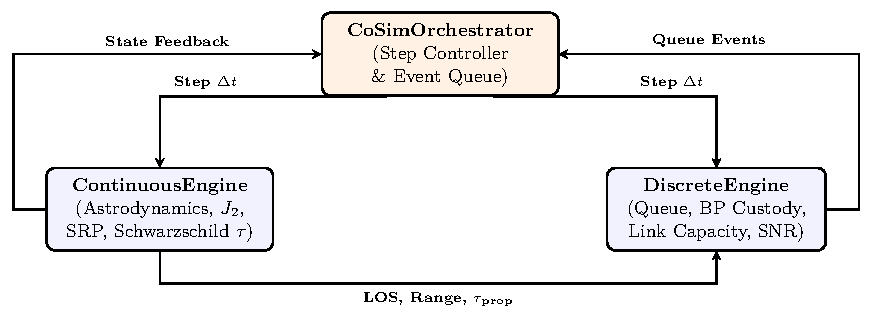
\includegraphics[width=0.88\textwidth]{else_paper/fig_architecture.pdf}\\[1pt]
        {\fontsize{6.5pt}{7.5pt}\selectfont \textbf{Flight Engine (Continuous)} $\;\longleftrightarrow\;$ \textbf{Network Engine (ns-3)}}\\[2pt]

        \begin{tcolorbox}[highlightbox]
            {\color{darkCyan}\textbf{Smart Step Controller: Zoom In \& Zoom Out:}}
            \begin{itemize}[leftmargin=8pt, itemsep=2pt, topsep=1pt]
                \item \textbf{In Quiet Cruise:} Takes large strides in time (up to 1 hour) to run simulations at blazing speed.
                \item \textbf{Near Critical Events:} Automatically zooms in to split-second precision right as a satellite enters or leaves planetary shadow.
                \item \textbf{Zero Boundary Delay:} Catches every contact start and end with \textbf{0.00 ms error} without burning CPU time.
            \end{itemize}
        \end{tcolorbox}

        \vspace{2pt}
        \begin{tcolorbox}[enhanced, colback=green!5, colframe=greenAccent, boxrule=1pt, arc=3pt, left=4pt, right=4pt, top=3pt, bottom=3pt]
            {\color{greenAccent}\textbf{True Time-Weighted Accuracy:}}
            \begin{itemize}[leftmargin=8pt, itemsep=1.5pt, topsep=1pt]
                \item Measures real orbital error across continuous mission time rather than artificially favoring fixed snapshots.
                \item Ensures flight tracking errors do not corrupt network throughput calculations.
            \end{itemize}
        \end{tcolorbox}

        \vspace{3pt}
        \begin{tcolorbox}[enhanced, colback=white, colframe=electricCyan, boxrule=1pt, arc=3pt, left=4pt, right=4pt, top=3pt, bottom=3pt]
            \begin{minipage}[c]{0.26\textwidth}
                \centering
                
\includegraphics[width=\linewidth]{qrcode_preprint.pdf}
            \end{minipage}%
            \hfill
            \begin{minipage}[c]{0.71\textwidth}
                {\fontsize{7pt}{8.5pt}\selectfont \color{darkCyan}\textbf{Full Paper \& Engine Source Code:}}\\[1pt]
                {\fontsize{6pt}{7.2pt}\selectfont Scan QR code for complete manuscript, benchmark data, and engine code repository:}\\[1.5pt]
                {\fontsize{5.2pt}{6.2pt}\selectfont \color{darkCyan}\texttt{github.com/PandiaJason/SPICE-ns-Project}}
            \end{minipage}
        \end{tcolorbox}
    \end{tcolorbox}
\end{minipage}

% ==============================================================================
% PAGE 2: BENCHMARK EVIDENCE, PARETO OPTIMALITY, AND NS-3 BLUEPRINTS
% ==============================================================================
\newpage

% Header Banner Page 2
\begin{tcolorbox}[enhanced, colback=spaceNavy, colframe=electricCyan, boxrule=1.5pt, arc=5pt,
    left=9pt, right=9pt, top=5pt, bottom=5pt]
    \begin{minipage}[c]{0.75\textwidth}
        {\fontsize{7.5pt}{9pt}\selectfont \color{electricCyan}\textbf{ICNS3 - 2026 LIGHTNING TALK --- PART 2: RESULTS \& ARCHITECTURAL BLUEPRINTS}}\\[2pt]
        {\fontsize{12pt}{14pt}\selectfont \color{white}\textbf{Benchmark Proof: Pareto Frontiers \& Blueprints for ns-3 Deep-Space Simulation}}\\[2pt]
        {\fontsize{7.5pt}{9.5pt}\selectfont \color{gray!30}Demonstrating synchronization performance across Mars Occultation, High-Speed Flyby, and 13-day Lunar missions.}
    \end{minipage}%
    \hfill
    \begin{minipage}[c]{0.23\textwidth}
        \centering
        \begin{tcolorbox}[colback=pillBg, colframe=greenAccent, boxrule=0.8pt, arc=3pt, left=4pt, right=4pt, top=3pt, bottom=3pt]
            \centering
            {\fontsize{7pt}{8pt}\selectfont \color{greenAccent}\textbf{BENCHMARK PROVEN}}\\[1pt]
            {\fontsize{6.5pt}{7.5pt}\selectfont \color{white} Speedup: \textbf{5.4$\times$ to 9.9$\times$ Faster}}\\
            {\fontsize{6.5pt}{7.5pt}\selectfont \color{white} Timing Error: \textbf{0.0 ms} vs 32.7 s}\\
            {\fontsize{6.5pt}{7.5pt}\selectfont \color{pillCyan} Scalability: \textbf{500 Spacecraft}}
        \end{tcolorbox}
    \end{minipage}
\end{tcolorbox}

\vspace{0.1cm}

% Top Row: Visual Benchmarks (Left) & Metrics Table + Scalability (Right)
\begin{minipage}[t]{0.48\textwidth}
    \begin{tcolorbox}[posterbox, title=4. Visual Proof: The Sweet Spot of Speed and Accuracy, height=9.0cm]
        \centering
        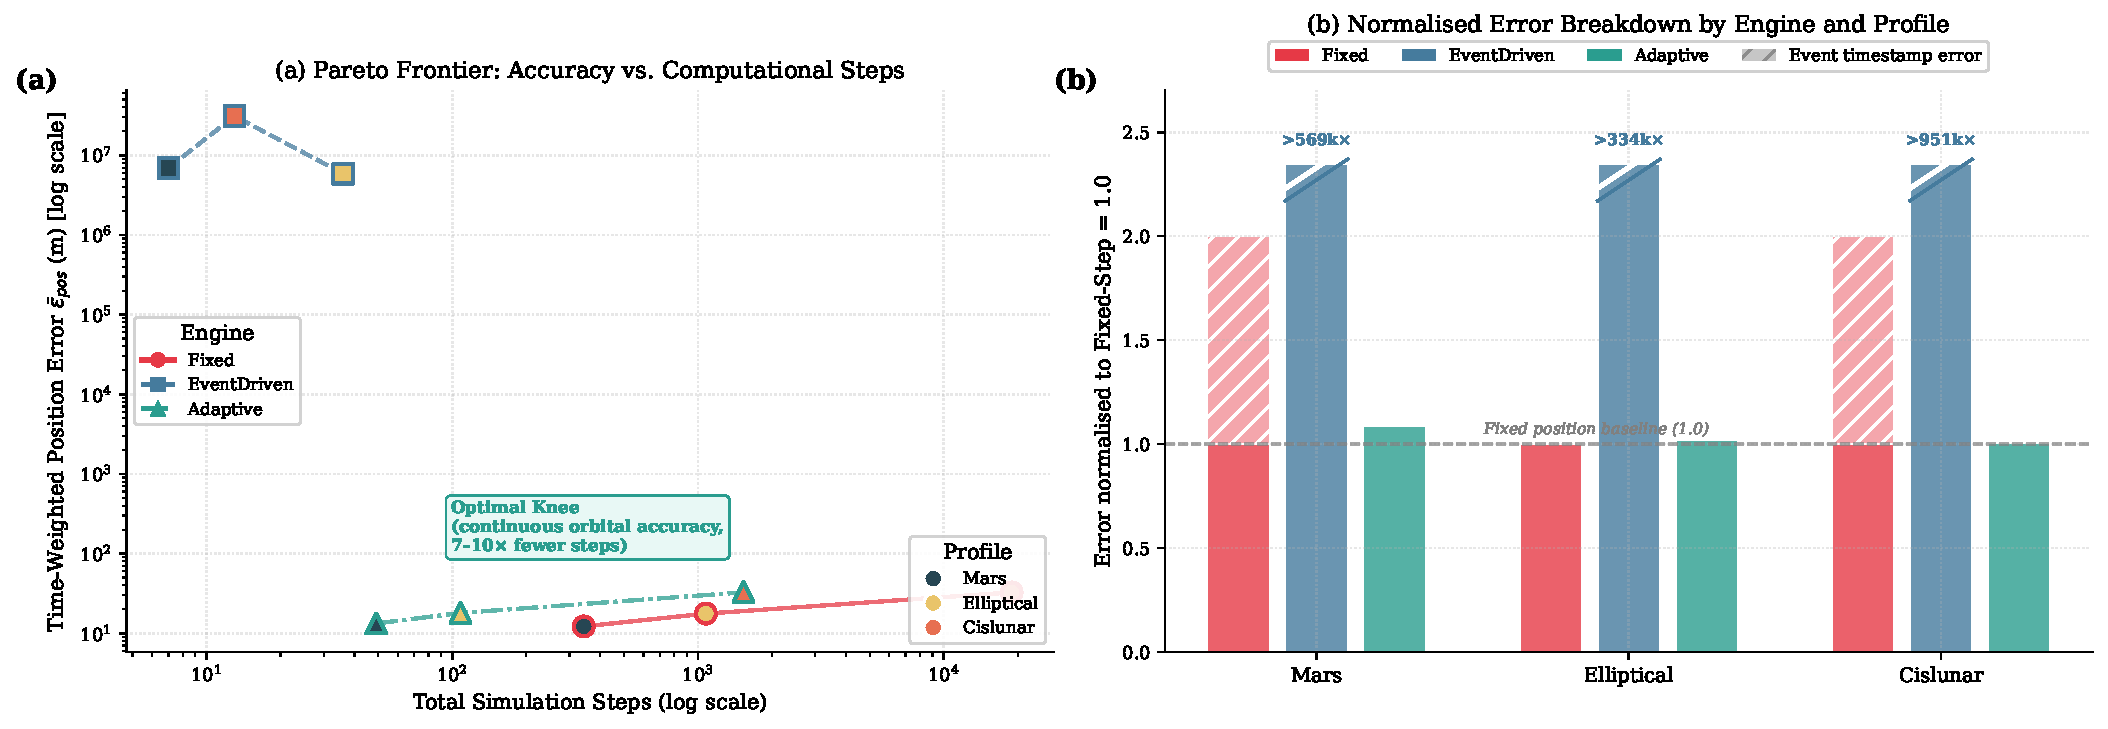
\includegraphics[width=\textwidth,height=4.1cm,keepaspectratio]{else_paper/fig3_accuracy_panel.pdf}\\[2pt]

        \begin{tcolorbox}[highlightbox]
            {\scriptsize \textbf{Key Takeaways from the Data:}}
            \begin{itemize}[leftmargin=8pt, itemsep=2pt, topsep=1pt]
                \item \textbf{The Optimal Knee:} Our adaptive engine runs \textbf{5.4× to 9.9× faster} than fixed stepping, using up to 10× fewer compute steps with \textbf{zero timing error} ($0.0\text{ ms}$).
                \item \textbf{Stopping the Ghost Drift:} Traditional event simulators accumulate \textbf{over 30,970 kilometers} of ghost drift during radio silence. Our adaptive engine continuously tracks gravity in the background, keeping errors bounded to \textbf{meters} (matching NASA SPICE standards).
            \end{itemize}
        \end{tcolorbox}
    \end{tcolorbox}
\end{minipage}%
\hfill
\begin{minipage}[t]{0.50\textwidth}
    \begin{tcolorbox}[posterbox, title=5. Benchmark Performance \& Real-World Consequences, height=9.0cm]
        {\centering{\scriptsize \textbf{Benchmark Comparison Across Three Space Profiles}}\par}
        \vspace{2pt}
        \noindent\resizebox{\linewidth}{!}{
        \begin{tabular}{l l r r r}
            \toprule
            \textbf{Scenario} & \textbf{Metric} & \textbf{Fixed-Step (60s)} & \textbf{Event-Driven} & \textbf{Adaptive Multi-Rate} \\
            \midrule
            \textbf{Mars Occultation} & Compute Time (Steps) & 0.09 s (343 steps) & 0.005 s (7 steps) & \textbf{0.017 s (49 steps)} \\
            (Passing behind planet)   & Position Drift Error & 12.2 meters         & 6,940 kilometers    & \textbf{13.3 meters} \\
                                      & Boundary Delay Error & 29.9 seconds        & 0.00 ms             & \textbf{0.00 ms} (\textbf{5.4$\times$ faster}) \\
            \midrule
            \textbf{Molniya Orbit}    & Compute Time (Steps) & 0.28 s (1,077 steps)& 0.015 s (36 steps)  & \textbf{0.035 s (108 steps)} \\
            (High-speed Earth flyby)  & Position Drift Error & 17.6 meters         & 5,890 kilometers    & \textbf{18.0 meters} \\
                                      & Boundary Delay Error & 0.00 ms             & 0.00 ms             & \textbf{0.00 ms} (\textbf{8.1$\times$ faster}) \\
            \midrule
            \textbf{13-Day Moon NRHO} & Compute Time (Steps) & 5.03 s (18,901 steps)& 0.012 s (13 steps) & \textbf{0.51 s (1,532 steps)} \\
            (Long lunar cruise)       & Position Drift Error & 32.6 meters         & 30,970 kilometers   & \textbf{32.7 meters} (accurate) \\
                                      & Boundary Delay Error & 32.7 seconds        & 0.00 ms             & \textbf{0.00 ms} (\textbf{9.9$\times$ faster}) \\
            \bottomrule
        \end{tabular}
        }

        \vspace{2pt}
        \begin{minipage}[c]{0.42\textwidth}
            \centering
            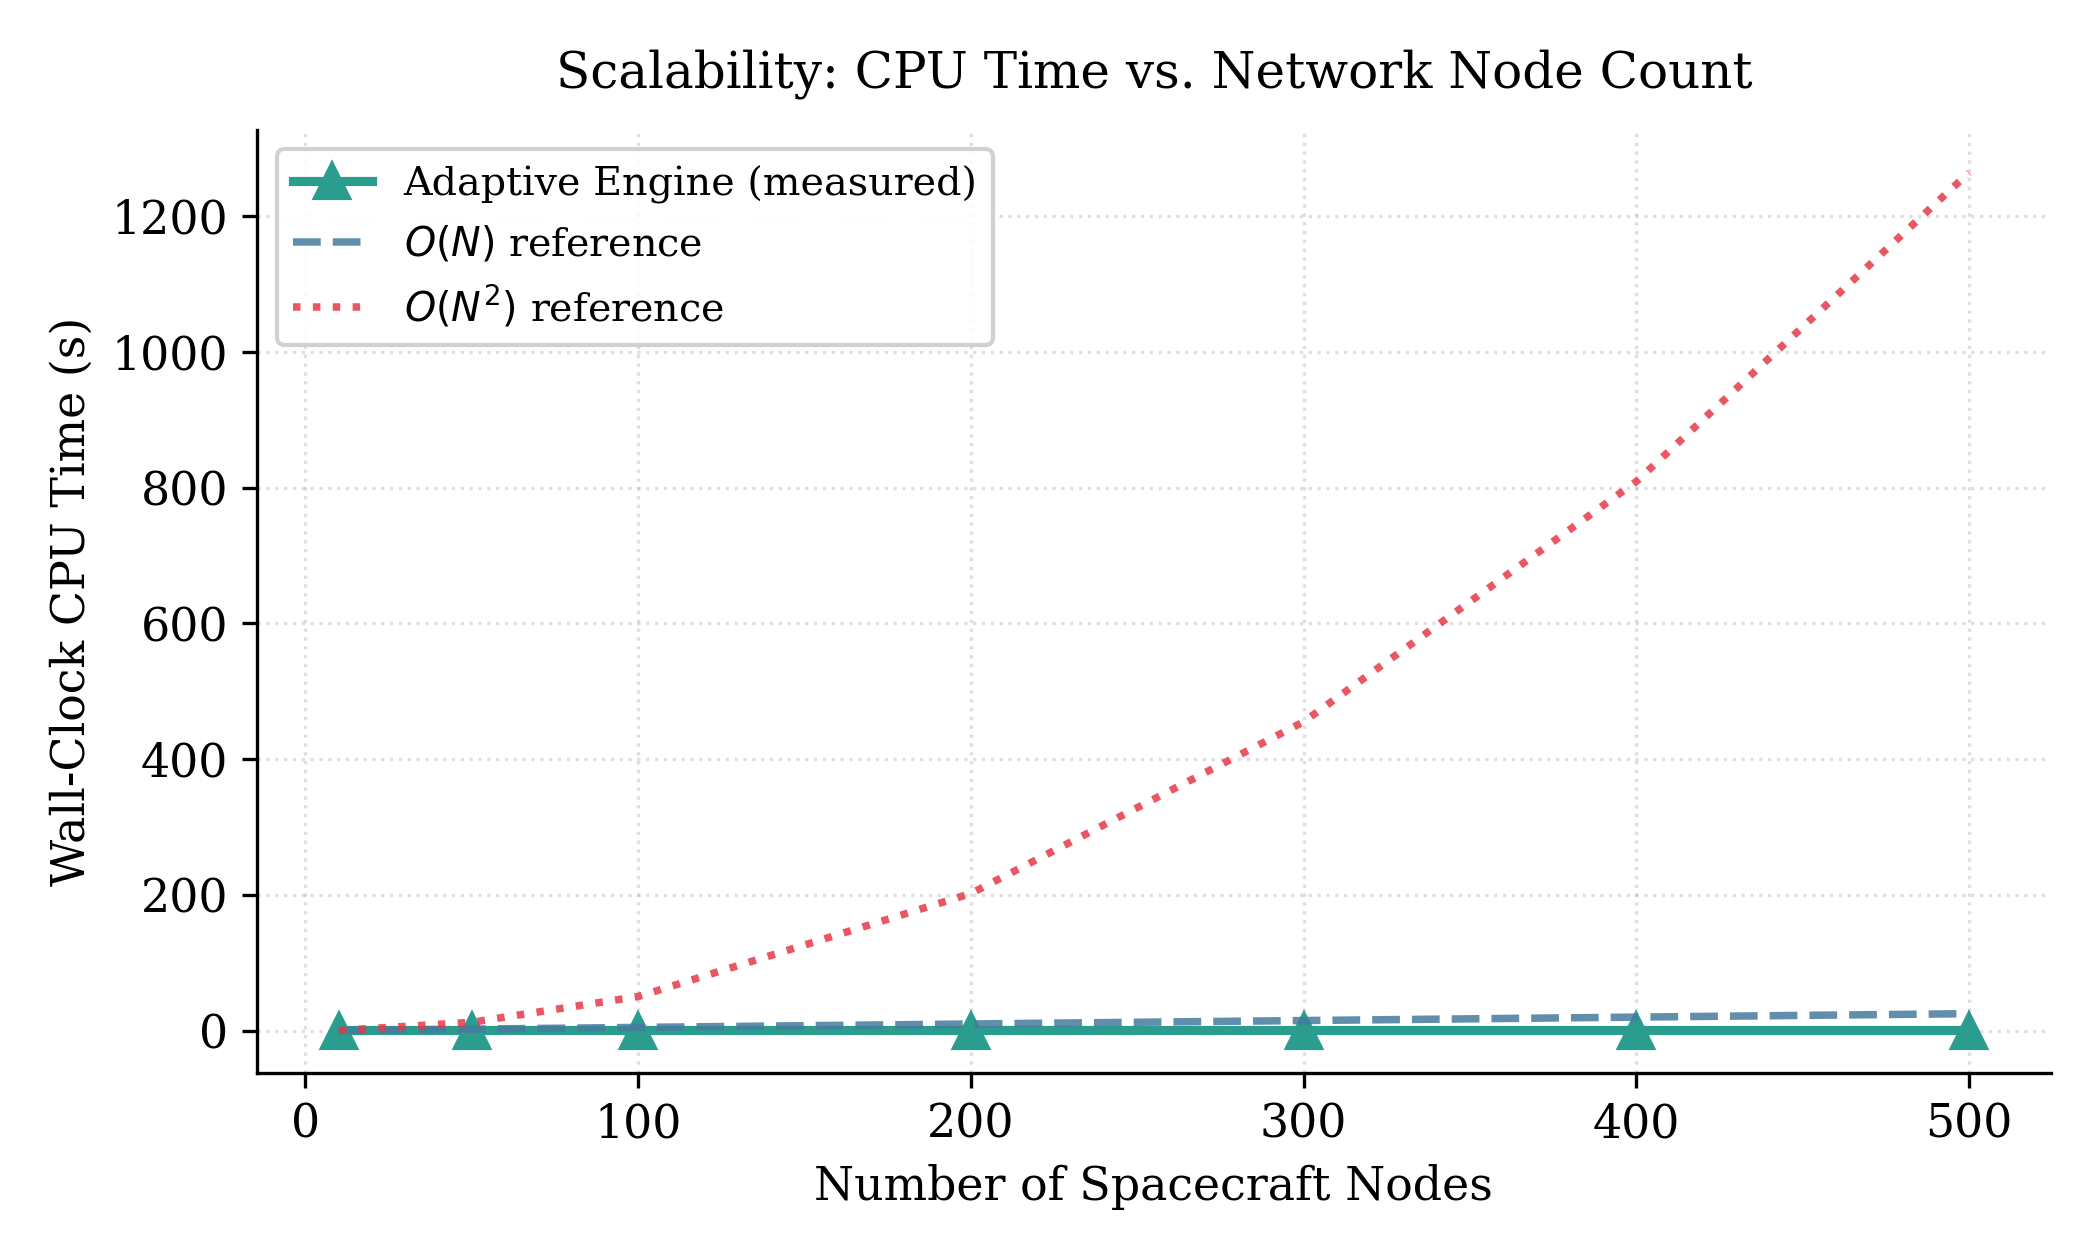
\includegraphics[width=\textwidth,height=2.2cm,keepaspectratio]{else_paper/fig5_scalability.png}\\[1pt]
            {\fontsize{5.5pt}{6.5pt}\selectfont \textbf{Scalability (10--500 Spacecraft):} Simulates 500 space nodes in just 6.35 seconds with zero software lockups.}
        \end{minipage}%
        \hfill
        \begin{minipage}[c]{0.56\textwidth}
            \begin{tcolorbox}[amberbox, left=3pt, right=3pt, top=2.5pt, bottom=2.5pt]
                {\fontsize{6.8pt}{8pt}\selectfont \color{accentAmber}\textbf{What Happens in the Real World If Simulators Lie?}}
                \begin{itemize}[leftmargin=7pt, itemsep=0.8pt, topsep=1pt]
                    {\fontsize{5.8pt}{7.0pt}\selectfont
                    \item \textbf{False Connection Predictions:} A 30,000 km position error alters calculated radio signal strength by \textbf{up to 14 dB}, falsely reporting high-speed links during total blackout.
                    \item \textbf{Phantom Data Speeds:} Stale positions cause the simulator to schedule peak transmission (20 Mbps) when the actual channel is dead (0 Mbps).
                    \item \textbf{Panic Retransmission Storms:} Underestimating delay makes network timers expire prematurely, triggering storms of duplicate packets.
                    \item \textbf{Catastrophic Lost Science Data:} Falsely assuming data is flowing hides buffer overflows, permanently deleting precious space photos.
                    }
                \end{itemize}
            \end{tcolorbox}
        \end{minipage}
    \end{tcolorbox}
\end{minipage}

\vspace{0.06cm}

% Bottom Row: 3 Strategic Blueprints for ns-3 Community
\begin{minipage}[t]{0.32\textwidth}
    \begin{tcolorbox}[posterbox, title=Blueprint 1: Aim Where the Spacecraft Will Be, height=5.0cm]
        {\color{darkCyan}\textbf{In-Flight Light-Time Solver:}}
        \begin{itemize}[leftmargin=8pt, itemsep=2pt, topsep=1pt]
            \item \textbf{Today's Limitation:} ns-3 calculates signal delay based on where the spacecraft was when transmission started.
            \item \textbf{Our Proposal:} Teach ns-3 to solve where the moving target will actually be when the signal arrives minutes or hours later across the solar system.
            \item Prevents massive link geometry errors during long interplanetary flights.
        \end{itemize}
    \end{tcolorbox}
\end{minipage}%
\hfill
\begin{minipage}[t]{0.32\textwidth}
    \begin{tcolorbox}[posterbox, title=Blueprint 2: Smart Early-Warning Alarms, height=5.0cm]
        {\color{darkCyan}\textbf{Boundary Event Guarding:}}
        \begin{itemize}[leftmargin=8pt, itemsep=2pt, topsep=1pt]
            \item \textbf{Today's Limitation:} Simulators force computers to take millions of tiny fixed steps just to watch for when a satellite dips behind a planet.
            \item \textbf{Our Proposal:} Introduce smart look-ahead triggers so the simulator speeds through quiet space and only slows down at exact threshold crossings.
            \item Eliminates 30-second timing delays without burning CPU power.
        \end{itemize}
    \end{tcolorbox}
\end{minipage}%
\hfill
\begin{minipage}[t]{0.33\textwidth}
    \begin{tcolorbox}[posterbox, title=Blueprint 3: Deep-Space Multi-Clock Sync, height=5.0cm]
        {\color{darkCyan}\textbf{Relativistic Time Adjustment:}}
        \begin{itemize}[leftmargin=8pt, itemsep=2pt, topsep=1pt]
            \item \textbf{Today's Limitation:} ns-3 uses a single global clock that assumes time ticks identically everywhere.
            \item \textbf{Our Proposal:} Support local spacecraft clocks that adjust for Einstein's gravitational and speed time dilation near massive planets.
            \item Ensures accurate packet timestamps between planetary orbiters and ground stations.
        \end{itemize}
    \end{tcolorbox}
\end{minipage}

\vspace{0.08cm}

% Footer Banner
\begin{tcolorbox}[enhanced, colback=spaceNavy, colframe=electricCyan, boxrule=1.2pt, arc=4pt,
    left=8pt, right=8pt, top=3.5pt, bottom=3.5pt]
    \centering
    {\fontsize{7.5pt}{9pt}\selectfont \color{white}
    \textbf{Full Manuscript Under Peer Review:} \textit{``The Limits of Discrete-Event Synchronization in Interplanetary Network Simulation: A Critical Review of Co-Simulation Fidelity''}, submitted to \textbf{\color{pillCyan}Simulation Modelling Practice and Theory (Elsevier)}.}\\[2pt]
    {\fontsize{6.8pt}{8.2pt}\selectfont \color{gray!30}
    \textbf{Open-Source Engine \& Benchmark Artifacts:} \texttt{https://github.com/PandiaJason/SPICE-ns-Project/tree/main/Adaptive-Multi-Rate-Co-Simulation-Engine} \quad $\vert$ \quad
    \textbf{Presenter:} Jason Pandian (\texttt{pandiajason@gmail.com}) \quad $\vert$ \quad \textbf{ICNS3 - 2026 Lightning Talk}}
\end{tcolorbox}

\end{document}
